\adparagraph{Kendall Tau Distance}
Looking at Figure \ref{fig:kendalldistance} we can see the results of the SFD test. As mentioned in Section \ref{sec:distance}\note{mention this} the distanced measures have a score between 0 and 1 where 0 correspond to equal lists and 1 that the lists are reverse of each other. There is a third case as the method we uses find an average approach meaning that if we have completely disjoint lists the distance score will be 0.78.

A general trend when looking at the graph is that all the methods follow the same curve where there is a somewhat large difference of around 0.04 between group sizes 4 and 8. However as the groups grow the increase in the KTD fades out and becomes very low and the difference between 20 and 40 is approximately 0.006. 

Looking at the approaches individually AVG clearly scores the highest. The reason is that AVG disregards the item ranks in the top-k lists and aggregates them based on the average rating between the group members instead.  
   
Next we have SF. This is surprising because, within the information retrieval domain, SF usually perform notably better than BC does. \note{Find cite for this} We do not have a reasonable explanation for why this is the case, but we expect it to have something to do with SF placing items placed using a median like approach which may have same issues as average.

Lastly performing best and somewhat equal we have BC and MC. Worth noting is that when the groups are small MC performers slightly better than BC, but already at group size 8 BC out scales MC.

\begin{figure}[H]
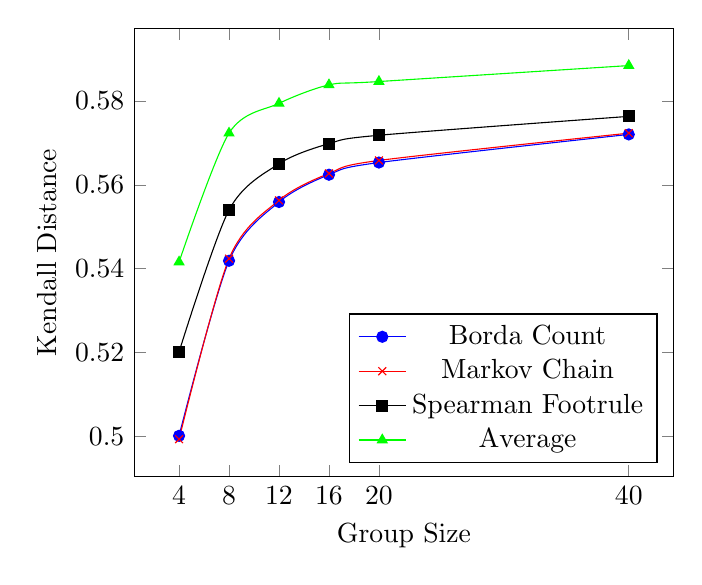
\begin{tikzpicture}
    \begin{axis}[
        xlabel=Group Size,
        ylabel=Kendall Distance,
        xtick = {4,8,12,16,20,40},
        legend pos=south east]
    \addplot[smooth,mark=*,blue] plot coordinates {
        (4,0.5002)
        (8,0.5419)
        (12,0.5559)
        (16,0.5624)
        (20,0.5653)
        (40,0.572)
    };
    \addlegendentry{Borda Count}

    \addplot[smooth,color=red,mark=x] plot coordinates {
            (4,0.4994)
            (8,0.5424)
            (12,0.5563)
            (16,0.5627)
            (20,0.5658)
            (40,0.5723)
        };
    \addlegendentry{Markov Chain}
    
        \addplot[smooth,color=black,mark=square*] plot coordinates {
            (4,0.5202)
            (8,0.554)
            (12,0.565)
            (16,0.5698)
            (20,0.5718)
            (40,0.5763)
        };
    \addlegendentry{Spearman Footrule}
    
    \addplot[smooth,color=green,mark=triangle*] plot coordinates {
            (4,0.5416)
            (8,0.5723)
            (12,0.5794)
            (16,0.5838)
            (20,0.5846)
            (40,0.5884)
        };
    \addlegendentry{Average}
    
    \end{axis}
\end{tikzpicture}
\caption{Results using Kendall Tau distance} \label{fig:kendalldistance}
\end{figure}

